\section{More about errors and sample size}

\nl \textbf{\color{eblue}Motivational example: } $X$ equals the breaking strength of a steel bar. If the bar is manufactured by Process I, it is known $X \sim N(50,\;36).$

\nl We now have Process II and it is hoped that the steel is 10\% stronger. i.e. $X \sim N(55,\;36)$.

\nl Our test? $$H_0 : \mu_I = 50 \hspace{1in} H_a : \mu_{II} = 55$$
{\red{Okay... we can't really test \say{this}}}

\nl But we can construct a hypothetical test where if $H_a$ is true, we can minimize (or control) both the Type I and Type II errors.

\nl For the sake of concrete-ness, set $n=16$. Then,
$$\sigma_{\Xbar}^2 = \frac{36}{16} \wideand \sigma_{\Xbar} = 1.5$$
\begin{center}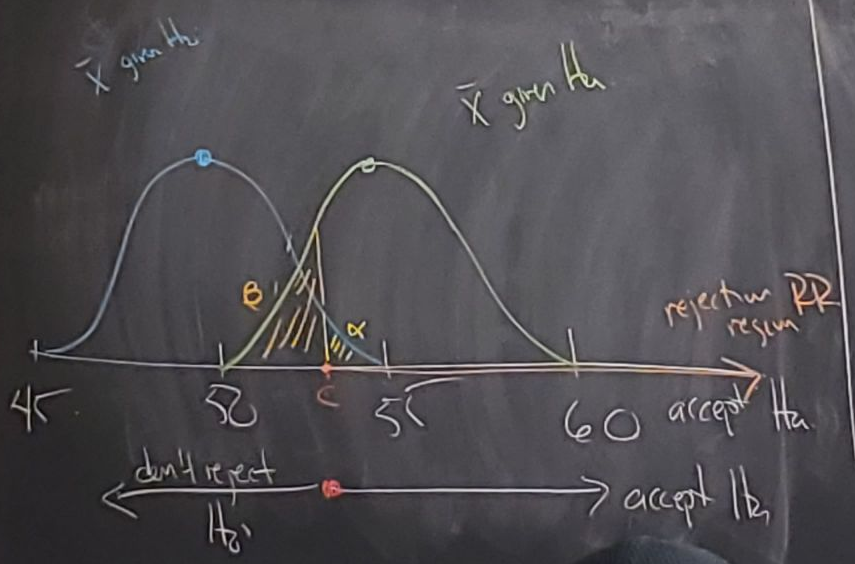
\includegraphics[width=6.5in]{2_25_1.png}\end{center}
$$\alpha = \P{\text{Type I}} \qquad H_0 : \mu = 50 \qquad H_a : \mu < 50$$
On the other hand, given $\alpha$, we can also see
$$\beta = \P{\text{Type II}} = \P{\text{accept } H_0 \text{ when } H_a \text{ is true}}$$


\nl Given $\alpha$, we can find $c$.
\begin{align*}
    \alpha &= \P{\Xbar > C \mid H_0}\\
    &= \P{\frac{\Xbar -{\color{blue}50}}{1.5} > \frac{C-{\color{blue}50}}{1.5}}
\end{align*}
and
\begin{align*}
    \beta &= \P{\Xbar < C \mid H_a}\\
    &= \P{\frac{\Xbar - {\color{ggreen}55}}{1.5} < \frac{C-{\color{ggreen}55}}{1.5}} 
\end{align*}
For fixed $n=16$, usually choose $\alpha$ small.
$$\alpha = \P{\Xbar -50 > 2\sigma_{\Xbar}} = 0.025$$%probably should be 1.960 instead of 2
Then $C = 50 + 2(1.5) = 53$ and
\begin{align*}
    \beta &= \P{\Xbar < 53 \mid H_a}\\
    &= \P{\frac{\Xbar - 55}{1.5} < 1.33}\\
    &= 0.0918
\end{align*}
Note almost four times as likely to make a Type II error than a Type I error. Of course, decreasing $\alpha$ with increase $\beta$.
$$\alpha = 0.01 \quad \implies \quad Z\text{-score} = 2.33 \qquad (Z_{0.98})$$
$$c = 50 + 2.33 (1.5) = 53.495$$
\begin{align*}
    \beta &= \P{\Xbar < 53.495 \mid H_a}\\
    &= \P{Z < -1.003}\\
    &= 0.1587
\end{align*}
Again, we note that the only way to decrease \textit{both} $\alpha$ and $\beta$ is to crank up the $n$.

\disc Choosing sample size $n$. We consider the 1-sided test
$$H_0 : \mu = \mu_0 \hspace{1in} H_a : \mu > \mu_0$$
Fix $\alpha$ at the start.
\begin{align*}
    \alpha &= \P{\Xbar > C \text{ when } \mu = \mu_0}\\
    &= \P{Z > \frac{C-\mu_0}{\sigma / \sqrt{n}}}\\
    &= \P{Z > Z_{\alpha}} \qquad Z_{\alpha} = \frac{C-\mu_0}{\sigma/\sqrt{n}}
\end{align*}
But, as with the power function, we need to choose specific $\mu_a$'s to work with (e.g. $\mu_a = 55$).
\begin{align*}
    \beta &= \P{\Xbar < C \text{ when } \mu = \mu_a}\\
    &= \P{Z < \frac{C-\mu_a}{\sigma / \sqrt{n}}}\\%
    &= \P{Z < -Z_{\beta}} \quad \text{when}\quad -Z_{\beta} = \frac{C-\mu_{\alpha}}{\sigma/\sqrt{n}}
\end{align*}
2 equations in the 2 unknows, $C,\;n$
$$C = \mu_0 + Z_{\alpha} \frac{\sigma}{\sqrt{n}} \wideand C = \mu_a - Z_{\beta} \frac{\sigma}{\sqrt{n}}$$
$$\mu + Z_{\alpha} \frac{\sigma}{\sqrt{n}} = \mu_a - Z_{\beta} \frac{\sigma}{\sqrt{n}} $$
Solve for $n$: 
$$(Z_{\alpha} + Z_{\beta})\frac{\sigma}{\sqrt{n}} = \mu_a - \mu_0$$
$$n = \frac{(Z_{\alpha} + Z_{\beta})^2 \sigma^2}{(\mu_a-\mu_0)^2}$$
Remark:
\begin{enumerate}[label=\textcircled{\raisebox{-1pt}{\arabic*}}]
    \item Of course all of this the fudge factor that we don't really know $\mu_a$.
    \item If we did $H_0 : \mu_0 = \mu_a$ and $H_a : \mu_0 > \mu_a$ we get the same formula for $n$. \say{sample size estimator for a one-sided $\alpha$-level test}
\end{enumerate}

\example* Back to the steel example

\nl If we decided at the start that we want $\alpha = \beta = 0.05$, what $n$ should we choose?

\nl For $\alpha = 0.05 \implies Z_{\alpha} = Z_{0.05} = 1.645$. Similarly for $\beta$, we need $Z_{\beta} = 1.645.$
Into our formula,
$$n = \pars{\frac{1.645+1.645}{\color{ggreen}55 \color{black} - \color{blue}50 \color{black}}}^2 \cdot 36 = \lceil 15.5867 \rceil = 16$$
Since we made $\alpha = \beta$ here, $C$ is the midpoint $C = \dfrac{55+50}{2} = 52.5$.
\begin{center}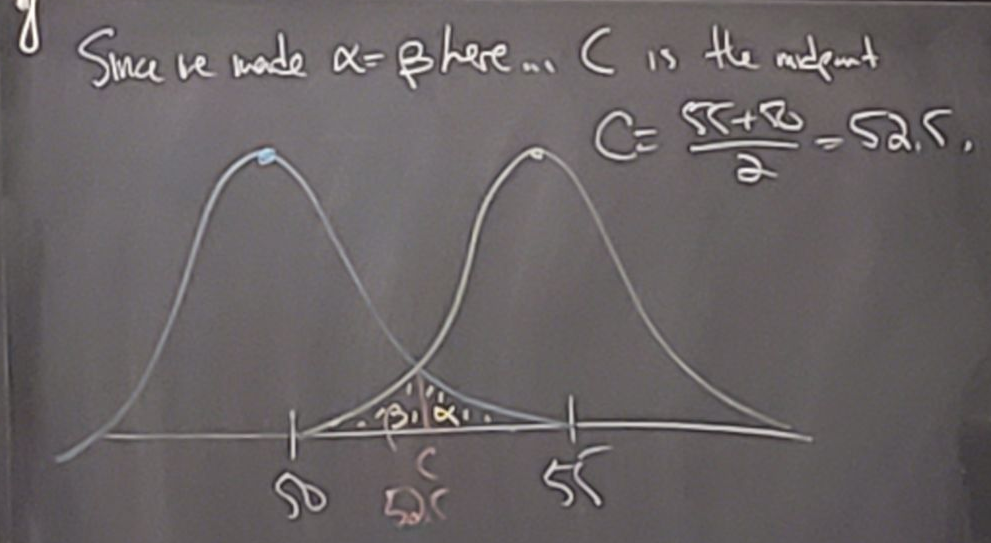
\includegraphics[width=4.5in]{2_25_2.png}\end{center}